

\section{Relative suffix tree}

The \emph{relative suffix tree} (\RCST) is a \CSTnpr{} of the
target sequence relative to a \CST{} of the reference sequence. It consists of
two major components: the relative FM-index with full functionality and the
\emph{relative} \LCP{} (\RLCP) \emph{array}. The optional relative select
structure can be generated or loaded from disk to speed up algorithms based on
forward searching. The \RLCP{} array is based on \RLZ{} parsing, while the
support for \nsv/\psv/\rmq{} queries is based on a minima tree over the
phrases.

\subsection{Relative \LCP{} array}

Given \LCP{} array $\mLCP[1,n]$, we define the \emph{differential} \LCP{}
\emph{array} $\mDLCP[1,n]$ as $\mDLCP[1] = \mLCP[1]$ and $\mDLCP[i] = \mLCP[i]
- \mLCP[i-1]$ for $i > 1$. If $\mBWT[i,j] = c^{j+1-i}$ for some $c \in
\Sigma$, then $\mLCP[\mLF(i)+1,\mLF(j)]$ is the same as $\mLCP[i+1,j]$, with
each value incremented by $1$ \cite{Fischer2009a}. This means
$\mDLCP[\mLF(i)+2,\mLF(j)] = \mDLCP[i+2,j]$, making the \DLCP{} array of a
repetitive text compressible with grammar-based compression
\cite{Abeliuk2013}.

We make a similar observation in the relative setting. If target sequence $S$
is similar to the reference sequence $R$, then their \LCP{} arrays should also
be similar. If there are long identical ranges $\mLCP_{R}[i,i+k] =
\mLCP_{S}[j,j+k]$, the corresponding \DLCP{} ranges $\mDLCP_{R}[i+1,i+k]$ and
$\mDLCP_{S}[j+1,j+k]$ are also identical. Hence we can use \RLZ{} parsing to
compress either the original \LCP{} array or the \DLCP{} array.

While the identical ranges are a bit longer in the \LCP{} array, we opt to
compress the \DLCP{} array, because it behaves better when there are long
repetitions in the sequences. In particular, assembled genomes often have long
runs of character $N$, which correspond to regions of very large \LCP{}
values. If the runs are longer in the target sequence than in the reference
sequence, the \RLZ{} parsing of the \LCP{} array will have many
mismatch characters. The corresponding ranges in the
\DLCP{} array typically consist of values $\set{-1, 0, 1}$, making them much
easier to compress.

We consider \DLCP{} arrays as strings over an integer alphabet and create an \RLZ{} parsing
of $\mDLCP_{S}$ relative to $\mDLCP_{R}$. After parsing, we switch to using
$\mLCP_{R}$ as the reference. The reference is stored in a
structure we call \slarray, which is a variant of \LCPbyte.
\cite{Abouelhoda2004}. Small values $\mLCP_{R}[i] < 255$ are stored in a byte
array, while large values $\mLCP_{R}[i] \ge 255$ are marked with a $255$ in the
byte array and stored separately. To quickly find the large values, we also
build a $\mrank_{255}$ structure over the byte array. The \slarray{} provides
reasonably fast random access and fast sequential access to the
underlying array.

The \RLZ{} parsing produces a sequence of phrases $w_{i} = (p_{i}, \ell_{i},
c_{i})$ (see Section~\ref{sect:rlz}; since we are using Cox et al.'s version, $c_{i}$ is now a string).
Because some queries involve decompressing an entire phrase, we limit the maximum phrase length to $1024$.
We also require that $\abs{c_{i}} > 0$ for all $i$, using the last character of the copied substring
as a mismatch if necessary.

Phrase lengths are encoded in the $W_{\ell}$ bitvector in the usual way. We convert the strings of mismatching
\DLCP{} values $c_{i}$ into strings of absolute \LCP{} values, append them into the mismatch array $W_{c}$, and
store the array as an \slarray. The mismatch values are used as \emph{absolute
samples} for the differential encoding.

To access $\mLCP_{S}[j]$, we determine the phrase $w_{i}$ as usual, and check whether we should return a mismatch character. If so, we compute which one using a prefix sum query on $L$, and return it.  If not, we determine the starting positions $p_{i}$ and $s_{i}$ of the phrase $w_{i}$ in the reference and the target, respectively. We can then compute the solution as
\begin{align*}
\mLCP_{S}[j] &= \mLCP_{S}[s_{i} - 1] + \sum_{k = s_{i}}^{j} \mDLCP_{S}[k] \\
&= \mLCP_{S}[s_{i} - 1] + \sum_{k = p_{i}}^{j'} \mDLCP_{R}[k] \\
&= \mLCP_{S}[s_{i} - 1] + \mLCP_{R}[j'] - \mLCP_{R}[p_{i} - 1],
\end{align*}
where $j' = p_{i} + j - s_{i}$.
Each \RLZ{} phrase ends with at least one mismatch character, so $\mLCP_{S}[s_{i} - 1]$ is readily available. After finding $\mLCP_{S}[j]$, accessing $\mLCP_{S}[j-1]$ and $\mLCP_{S}[j+1]$ is fast, as long as we do not cross phrase boundaries.


\paragraph{Example.}
Figure~\ref{fig:ex} shows an example reference sequence $R$ and target
sequence $S$, with their corresponding arrays $\SA$, $\LCP$, and $\DLCP$.
The single edit at $S[4]$ with respect to $R[4]$ may affect the positions
of suffixes $4$ and previous ones in $\SA$, although in general only a limited
number of preceding suffixes are affected. In our example, suffix $4$ moves
from position $7$ in $\SA_R$ to position $4$ in $\SA_S$, and suffix $3$ moves
from position $11$ in $\SA_R$ to position $10$ in $\SA_S$. Each suffix that
is moved from $\SA_R[i]$ to $\SA_S[j]$ may alter the values at positions $i$ 
or $i+1$ (depending on whether $j>i$ or $j<i$), as well as $j$ and $j+1$, of
$\LCP_S$. We have surrounded in rectangles the conserved regions in $\LCP_S$
(some are conserved by chance). Even some suffixes that 
are not moved may change their $\LCP$ values. In turn, each change in 
$\LCP_S[k]$ may change values $\DLCP_S[k]$ and $\DLCP_S[k+1]$.

After the change, we can parse $\DLCP_S$ into three phrases (with the copied
symbols surrounded by rectangles):
$(1,4,0)$, $(5,3,-2)$, $(6,2,-2)$, where the latter is formed by chance.
We represent this parsing as $W_c = \langle 1,0,0 \rangle$ (since we store the
absolute $\LCP_S$ values for the mismatches), $W_\ell = 100001000100$, and
$W_p = \langle 1,5,6 \rangle$ (or rather $W_r = \langle 0,-1,-4 \rangle$).

Let us compute $\LCP_S[j]$ for $j=8$. This corresponds to phrase number
$i = \rank(W_\ell,j) = 2$, which starts at position $s_i = \select(W_\ell,i)=6$
in $\LCP_S$. The corresponding position in $\LCP_R$ is $p_i = W_p[i] = 5$
(or rather $p_i = s_i + W_r[i] = 5$), and the mapped position $j$ is
$j' = p_i+j-s_i = 7$. Finally, $\LCP_S[s_i-1] = W_c[i-1]=1$.
According to our formula, then, we have
$\LCP_S[8] = \LCP_S[s_i-1] + \LCP_R[j'] - \LCP_R[p_i-1] = 1+2-1=2$.

\begin{figure}
\centerline{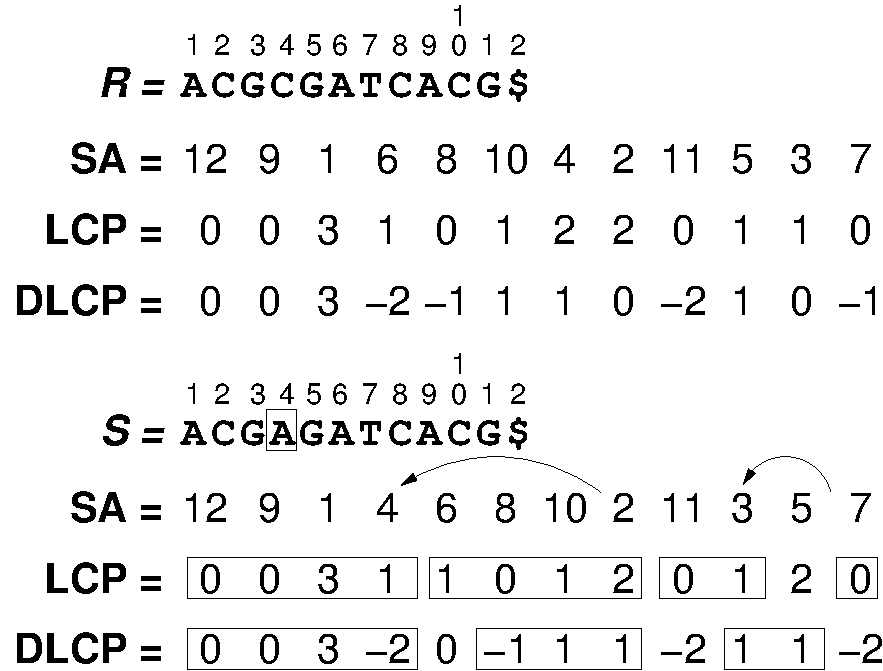
\includegraphics[width=0.4\textwidth]{ex.pdf}}
\caption{An example of our $\RLZ$ compression of $\DLCP$.}
\label{fig:ex}
\end{figure}

\subsection{Supporting \nsv/\psv/\rmq{} queries}

Suffix tree topology can be inferred from the \LCP{} array with range minimum
queries (\rmq) and next/previous smaller value (\nsv/\psv) queries
\cite{Fischer2009a}. Some suffix tree operations are more efficient
if we also support \emph{next/previous smaller or equal value} (\nsev/\psev)
queries \cite{Abeliuk2013}. Query $\mnsev(i)$ ($\mpsev(i)$) finds the next
(previous) value smaller than or equal to $\mLCP[i]$.

In order to support the queries, we build a $64$-ary \emph{minima tree} over
the phrases of the \RLZ{} parsing. Each leaf node stores the smallest \LCP{}
value in the corresponding phrase, while each internal node stores the
smallest value in the subtree. Internal nodes are created and stored in a
levelwise fashion, so that each internal node, except perhaps the rightmost
one of each level, has $64$ children.

We encode the minima tree as two arrays. The smallest \LCP{} values are
stored in $M_{\mLCP}$, which we encode as an \slarray. Plain array $M_{L}$
stores the starting offset of each level in $M_{\mLCP}$, with the leaves
stored starting from offset $M_{L}[1] = 1$. If $i$ is a minima tree node
located at level $j$, the corresponding minimum value is $M_{\mLCP}[i]$, the
parent of the node is $M_{L}[j+1] + \lfloor (i - M_{L}[j]) / 64 \rfloor$,
and its first child is $M_{L}[j-1] + 64 \cdot (i - M_{L}[j])$.

A range minimum query $\mrmq(sp,ep)$ starts by finding the minimal range of
phrases $w_{l}, \dotsc, w_{r}$ covering the query and the maximal range of
phrases $w_{l'}, \dotsc, w_{r'}$ contained in the query (note that $l \le l' \le
l+1$ and $r-1 \le r' \le r$). We then use the
minima tree to find the leftmost minimum value $j = M_{\mLCP}[k]$ in
$M_{\mLCP}[l',r']$, and find the leftmost occurrence $\mLCP[i] = j$ in phrase
$w_{k}$. If $l < l'$ and $M_{\mLCP}[l] \le j$, we decompress phrase $w_{l}$
and find the leftmost minimum value $\mLCP[i'] = j'$ (with $i' \ge sp$) in the
phrase. If $j' \le j$, we update $(i,j) \leftarrow (i',j')$. Finally we check
phrase $w_{r}$ in a similar way, if $r > r'$ and $M_{\mLCP}[r] < j$. The answer
to the range minimum query is $\mLCP[i] = j$, so we return
$(i,j)$.\footnote{The definition of the query only calls for the leftmost
minimum position $i$. We also return $\mLCP[i] = j$, because suffix tree
operations often need it.} Finally, the particular case where no phrase is
contained in $[sp,ep]$ is handled by sequentially scanning one or two phrases
in $\LCP$.

The remaining queries are all similar to each other. In order to answer query
$\mnsv(i)$, we start by finding the phrase $w_{k}$ containing position $i$,
and then determining $\mLCP[i]$. Next we scan the rest of the phrase to see
whether there is a smaller value $\mLCP[j] < \mLCP[i]$ later in the phrase. If
so, we return $(j,\mLCP[j])$. Otherwise we traverse the minima tree to find
the smallest $k' > k$ with $M_{\mLCP}[k'] < \mLCP[i]$. We decompress
phrase $w_{k'}$, find the leftmost position $j$ with $\mLCP[j] < \mLCP[i]$,
and return $(j,\mLCP[j])$.

